\documentclass[oneside,12pt]{memoir}

\usepackage[normalem]{ulem}
\usepackage{appendix}

\def\mychaplineone{Developer notes for}
\def\mychaplinetwo{ESGF Node Manager}
%\def\mychaplinethree{And Some More...}
\def\myauthone{Prashanth Dwarakanath}
\def\myauthtwo{Sasha Ames}
%\def\myauththree{Torgny Fax\'en}
\def\mypress{Earth System Grid Federation}
\usepackage{chengi}
\usepackage{biblatex}
\bibliography{thebib}
\DefineBibliographyStrings{english}{%
  bibliography = {References},
}
\def\nm{Node Manager{ }}
\def\vernum{March 18, 2014}
\setcounter{tocdepth}{2}
\thispagestyle{empty}
\titleGM
\chapterstyle{BlueBox}
\pagestyle{mystyle}
\begin{document}
\frontmatter
\hypertarget{mytocmarker}
\tableofcontents
\mainmatter
\setcounter{secnumdepth}{2}

%\section{Overview}

\chapter{Requirements and Features}

\section{Features List}

This list of features should not reflect specific design decisions meant as a means to satisfy any of the requirements, ie. it should be kept at a ``top'' level of abstraction.
\begin{itemize}
\item
\emph{Scalability}:  Federation can grow to NN nodes without degradation in performance
\item
Verify reachability via "heartbeat" 
\item
Maintain and propagate node map
\item
Provide statistics for dashboard
\item
Collect download statistics
\item
Add new node to federation
\item
Remove a node from federation
\item
Self-health check on each node
\item
Manage CSR request signing (requests/responses)
\item
Repository for ESGF component-specific config at project level, replicated to other nodes in project
\item
Eventual consistency guarantees, i.e. conflict resolution
\item
Node manager admin interface.  Allow admins to eg. sign certs, vet nodes,  
\end{itemize}

\section{Use Cases of ESGF node components}

\begin{center}
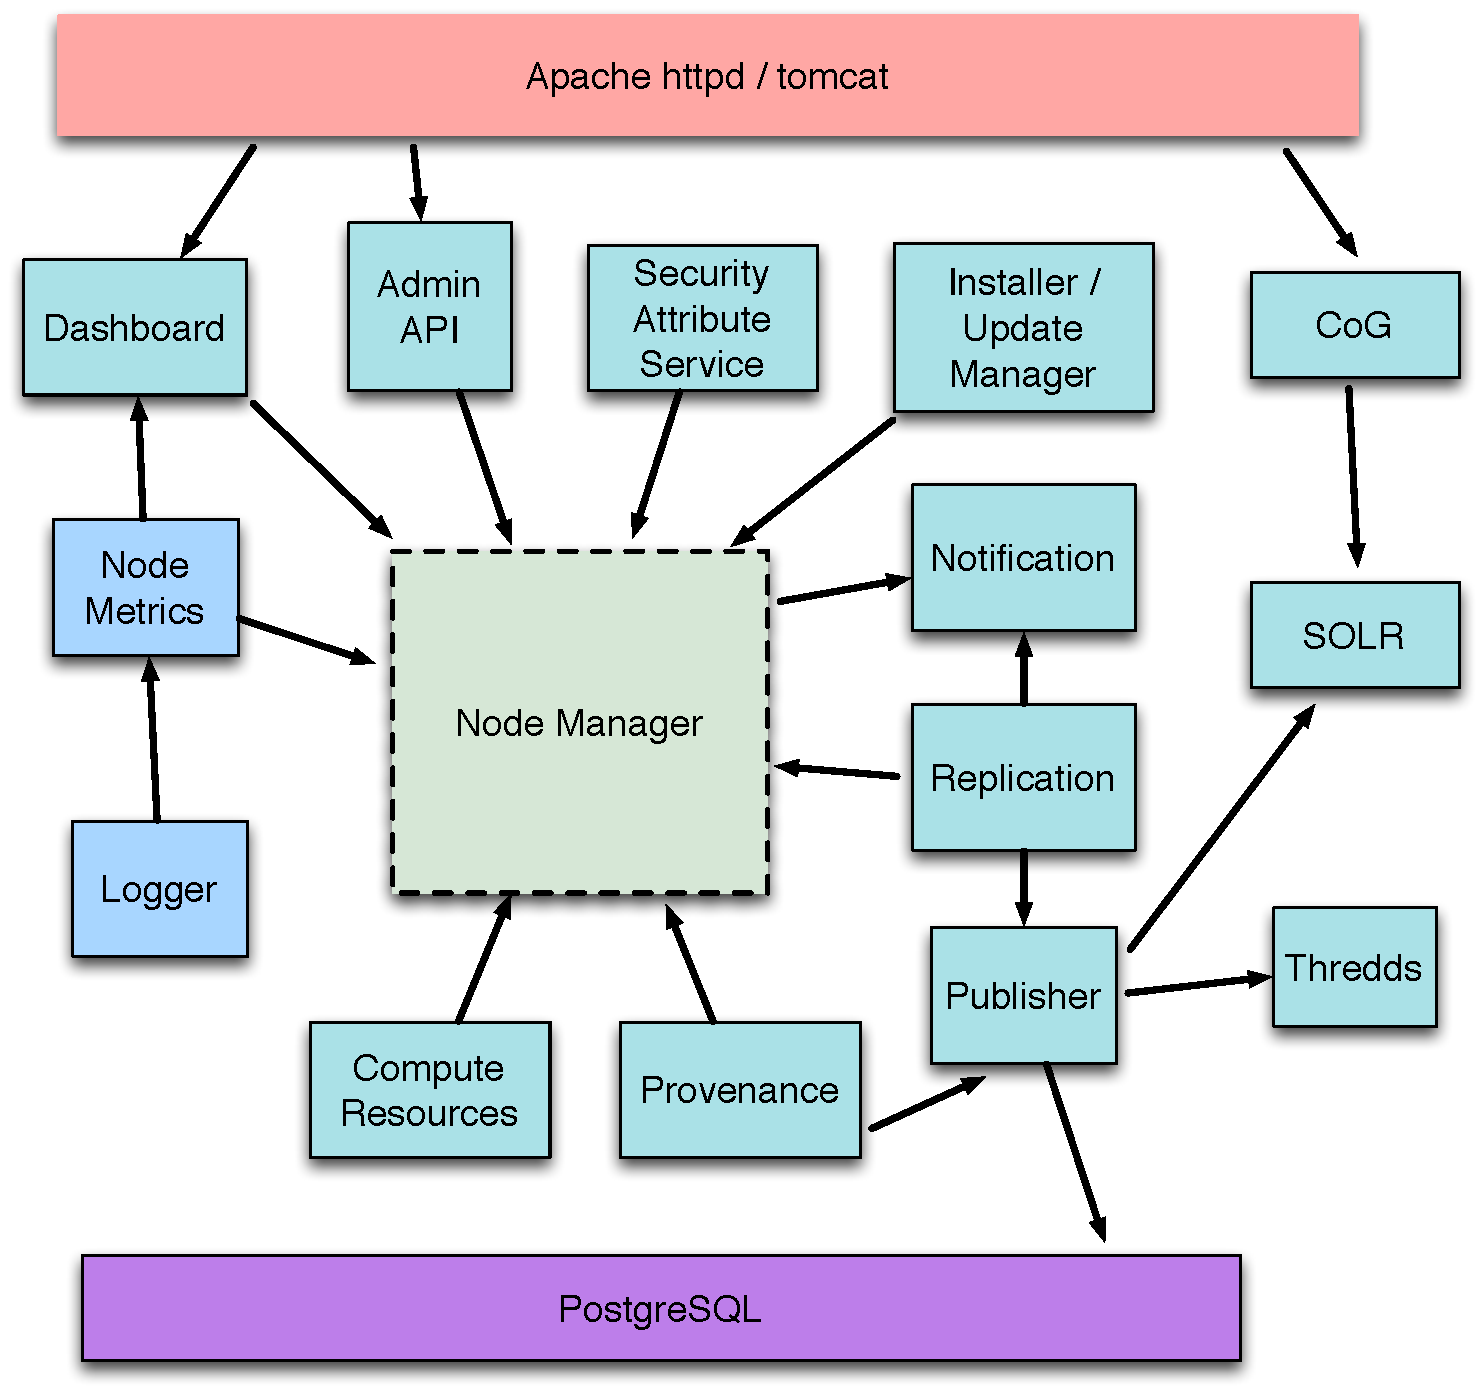
\includegraphics[width=\textwidth]{presentation/ESGF-node-components.pdf}

Figure 1:  relationship of Node Manager among other node components.  Many prominent or anticipated call paths between components are indicated.  Additional relationships are not necessarily shown.  
\end{center}


The following table lists various esgf components and an example of how the component would use the node manager to coordinate the service activities among several nodes.  \\
\\

\begin{tabular}{|c|l|}
\hline
Dashboard &  Manage consistent updates to registration.xml \\
\hline
Metrics & Coordinate metric metadata \\
\hline
Compute & Maintain repository of federated compute resources \\
\hline
Security & Replication of attributes for service failover \\
\hline
 IDP & Known providers list file \\
\hline
Update Manager & Consistent record of component versions \\
\hline
Notification & Push alert messages out to administrators / users \\
\hline
Replication & Data set version information \\
\hline
Publication & Consistent project-based configuration \\
\hline
Provenance & Consistent provenance metadata \\
\hline
Thredds & urls storage \\
\hline
SOLR / Search & Store shards lists \\
\hline
CoG & ??? \\
\hline
Logger & (metadata)? \\
\hline
\end{tabular}


\chapter{Name of the Solution}

A suggested name is \textbf{ESGF CH2}.  \textbf{C} for Client-server, \textbf{2H} for Hierarchical and Hybrid.  Our design choices depict a hierarchical solution, yet the design resembles P2P as well; thus, we may refer to it as a ``hybrid''.


\chapter{Solution Design}

\section{Design Considerations}
This section allows us to specific specific design decisions that support the desirable features of the Node Manager and steer the subsequent specific design patterns we use.

\begin{itemize}
\item 


We are interested in a hierarchical framework for node management rather than a pure p2p.  In this case nodes elect "SuperNodes" that perform additional tasks than "member-nodes".  Our goal for scalability is to have a balance of super vs member nodes to ensure that no SuperNode becomes oversubscribed.  Super-nodes operate at the "project" level.   
\item
A node that serves as the "SuperNode" for project A can be a member node for project B.  Super-nodes can serve in that role for multiple projects.    Configuring a node for eligibility for selection to become a SuperNode is voluntary, but important for the federation to have an "adequate" number of candidates.
\item
Vetting for a SuperNode. Hand-picked initial SuperNodes.  
\item
\sout{Member nodes pass messages. }  Member nodes are the endpoints for messages, ie. they will receive messages, reply to queries, or submit a limited set of requests.  

\item
Tree-based communication between SuperNodes and member nodes to reduce communication overheads, ie. avoid $n^2$ patterns.  We expect a ``wide'' tree with ``few" hops. Or consider filled-out binary tree structure (see below). 
\item 
Need to maintain backward compatibility with format of registration.xml etc, to not break existing parsers. 
\item
Member nodes can function independently from other SuperNodes. 
\end{itemize}







\section{System Architecture}



\begin{center}
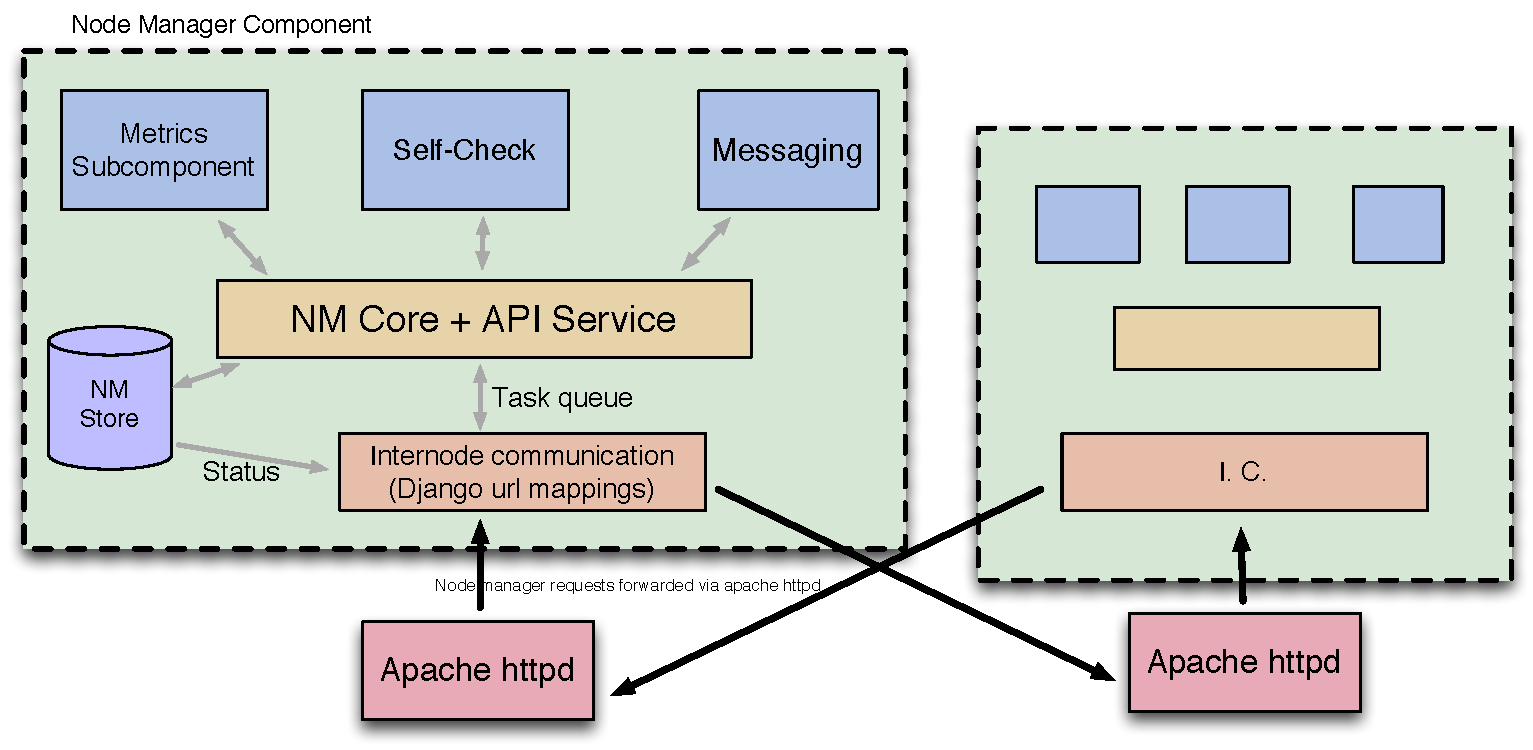
\includegraphics[width=\textwidth]{presentation/NM-design-v2.pdf}
Figure 2:  sub-components of the node manager and scheme for communication.  The node manager listens for connections/requests from other nodes via apache httpd and forwards (black arrows).  The messaging subcomponent determines need for communication and forwards requests to an esgf notification service (not shown).  Gray arrows show sub-component control flow.
\end{center}
\newpage

\subsection{Configuration Components}
\label{stow}

These are the main components of the solution with respect to configuration of the ESGF Node.
\begin{enumerate}
\item
\textbf{Local config file} 
\begin{enumerate}
\item Membership to projects.
\item Projects to serve as SuperNode/standby node (voluntary).


\end{enumerate}

\item
\textbf{Use of git:  }

\begin{itemize}
\item
Solves consistency issue as their protocols would handle race conditions between administrators submitting changes. 
\item
As they (github) are established, we should expect a highly available web service.  They have similar issues of failover to be highly available.
\item
Cons:
\begin{itemize}
\item
 Authentication / security issues: administrators making changes need push rights on github, requiring administration.  Eg., new administrator not granted permission in time for required change.
 \item
 Tricky to resolve site connectivity issues.  For instance, the key SuperNode might not be able to connect to github and retrieve an update.  Then, we need to administer a failover and have an alternate SuperNode handle that.  Failure to connect to github is a health check failure for a SuperNode, but the node can still be a member node (demotion).  
\end{itemize}
\end{itemize}


%Apache ZooKeeper seems to be a very promising fit for this role, so this component shall henceforth simply be refered to as ZooKeeper.
%After looking at ZooKeeper, we opt against incorporating  ZK in the node manager/ esgf software stack.  Instead we focus on implementing a component that loosely model's its communication style on ZK.  

\item \textbf{Files in central git repository}
\begin{enumerate}
\item Project specific config parameters. ex: thredds\_exclude\_variable list
\item Comprehensive list of SuperNodes for membernodes to consult.
\item Global configuration parameters for SuperNodes: limits for number of members to serve etc
\end{enumerate}
\item \textbf{Node Manager Service}
\begin{enumerate}
\item Membernodes service status
\item Current list of SuperNodes and the membernodes they serve (node map).
\end{enumerate}

%A component that serves as a `feeder', to the zookeeper. This would also provide an administrative interface to the node manager. This is the component of the node manager that is meant to be exposed to the federation, and not the ZooKeeper itself, and it includes the ESGF Node Manager API. Henceforth, this component shall simply be refered to as the node manager. The node manager will also be used by local admins, to generate requests for federation membership or certificate signing and allow SuperNode admins to ratify/sign these requests. The node manager would also be responsible for collection of metrics.

\end{enumerate}

\subsection{Communication handler subcomponent}
Communication occurs via https client to the apache server listening on the nodes.   The apache service pushes messages back to local API.   We assume a django-python implementation of the API.  Depending on what mechanism is selected for worker threads/queues.
 We describe the communication use cases and patterns below.  


\subsection{Metric subcomponent}

This subcomponent produces the metrics that appear on the dashboard or other UI.Much metric ``raw" data will be found in the log files.  A crawler procedure can gather stats from the logs.   The metric service can include aggregate information from the provenance collection system. \yellowline{Also, the currently built-in hooks to log realtime download activity etc would have to be refined to ensure greater accuracy and eliminate problems such as false positives/negatives.}
%An optional part of this is a centralized collection of the log data that can be queried efficiently.  We expect that this would be on data center SuperNodes.  

%Some metrics are based on node state managed by the "feeder" service.  The zookeeper DFS can be used as the metastore for metric metadata.  
\subsection{Self-check subcomponent}
This is a subcomponent of the node manager which is responsible for carrying out sanity checks at regular intervals, on itself. When it fails the sanity checks, it contacts the local node manager to flag itself ineligible to continue as a SuperNode/standby SuperNode/member node. When the node passes a subsequent sanity check, the self-check component contacts the local node manager, to flag itself ready for resumption of duties.  The self-check subcomponent would also use the messaging subcomponent, to send out alert notifications to the local admin, when sanity checks fail.

\subsubsection{Specific Checks}
Use this list to mention specific items on the node to use for self-check.
\begin{description}
\item[Mountpoints]  All TDS roots should be checked.  If they time out due to problem with the mount, the situation means the node is unhealthy.

\end{description}

\subsection{Messaging subcomponent}

The messaging subcomponent is used by the self-check subcomponent, to alert the local admin, when the state of the node changes, i.e. fails a sanity check,  clears one, after having been flagged down by previous checks, or a component configuration/metadata change fails a global write due to a race condition (i.e., multiple admins try to update a configuration simultaneously).  
  Messaging coordinates with esgf node notification service.

\subsection{NM Store}

File system or database usage to maintain node manager configuration.  The status of the node gets kept here so that information can be available to the django-based internode-api.



\section{Node manager capacities}
Each and every ESGF installation, irrespective of role, i.e. data, compute etc, would have the node manager as a component.  However, the node manager itself can function in different capacities. 
\begin{enumerate}
\item \textbf{Membernode}: This is the default capacity of a node manager. It cannot query other node manager instances and can only pass on validated messages. See Section~\ref{commcases} for more. A membernode can volunteer to be a SuperNode or a standby SuperNode.
\item \textbf{SuperNode}: This is a membernode which volunteered to function as a SuperNode and was vetted (by administrators). Responsible for querying nodes which it is responsible for.  A federation would have multiple SuperNoded which divide the workload among themselves. SuperNodes also perform aggregation of gathered metrics.  We refer to SuperNodes as "peers", while this relationship does not extend from SuperNodes to member nodes
\item \textbf{Standby SuperNode}: A standby SuperNode is a membernode which volunteered to function as a SuperNode when the number of SuperNodes in the federation falls below a predefined threshold. These nodes temporarily function as SuperNodes and return to being standy SuperNodes, when the SuperNode count stabilizes in the federation.
\end{enumerate}



\section{Communication use-cases}
\label{commcases}
%A bulk of internode communication is handled implicitly by ZooKeeper, releasing us from having to explicitly establish communication for tasks such as leader election, but the ZooKeeper is not exposed to the outside world. Instead, it is controlled/accessed with the node manager, which serves as both a controller for ZooKeeper itself, and also as a wrapper for ZooKeeper. This would need node manager instances to communicate with each other. Let's consider the types of communication between node manager instances.



\begin{enumerate}
\item \textbf{SuperNode to membernode}: metric queries, status queries, status change notification (standby to SuperNode, vice-versa, etc.)
\item \textbf{SuperNode to SuperNode}: Shoot the node in the head, in case of malfunction.  Shared information updates (See \ref{stow} item 3)  This communication can be carried out by network links between nodes on a MST.   In some circumstances a star topology is adequate.  
\item \textbf{SuperNode health checks}:  This communication unlike other SN communication can be $n^2$ as we expect the messages to be short and infrequent.   
\item \textbf{SuperNode join:}  SuperNodes should be able to be added while the federation is up and running without downtime.  Any SuperNode can handle this and propagate the node map.

\item \textbf{SuperNode extended leave-resume, reassign:}  We expect SuperNodes to be down for short term.  Extended leave is another issue. We maintain the SuperNode id rather than reassign to another node.  If the SuperNode moves hostname, that we accommodate in a similar fashion without federation downtime.  What is not handled is a permanent delete of a SuperNode.  


\item \textbf{Membernode to membernode}: passing on authenticated messages received from SuperNodes.  This communication is TBD (could be tree based using same principe as used within tree network of SuperNodes.) % (this is implicit in zookeeper's communication)  
\item \textbf{Membernode to SuperNode}: Pushing local config status etc.
\end{enumerate}

\begin{center}
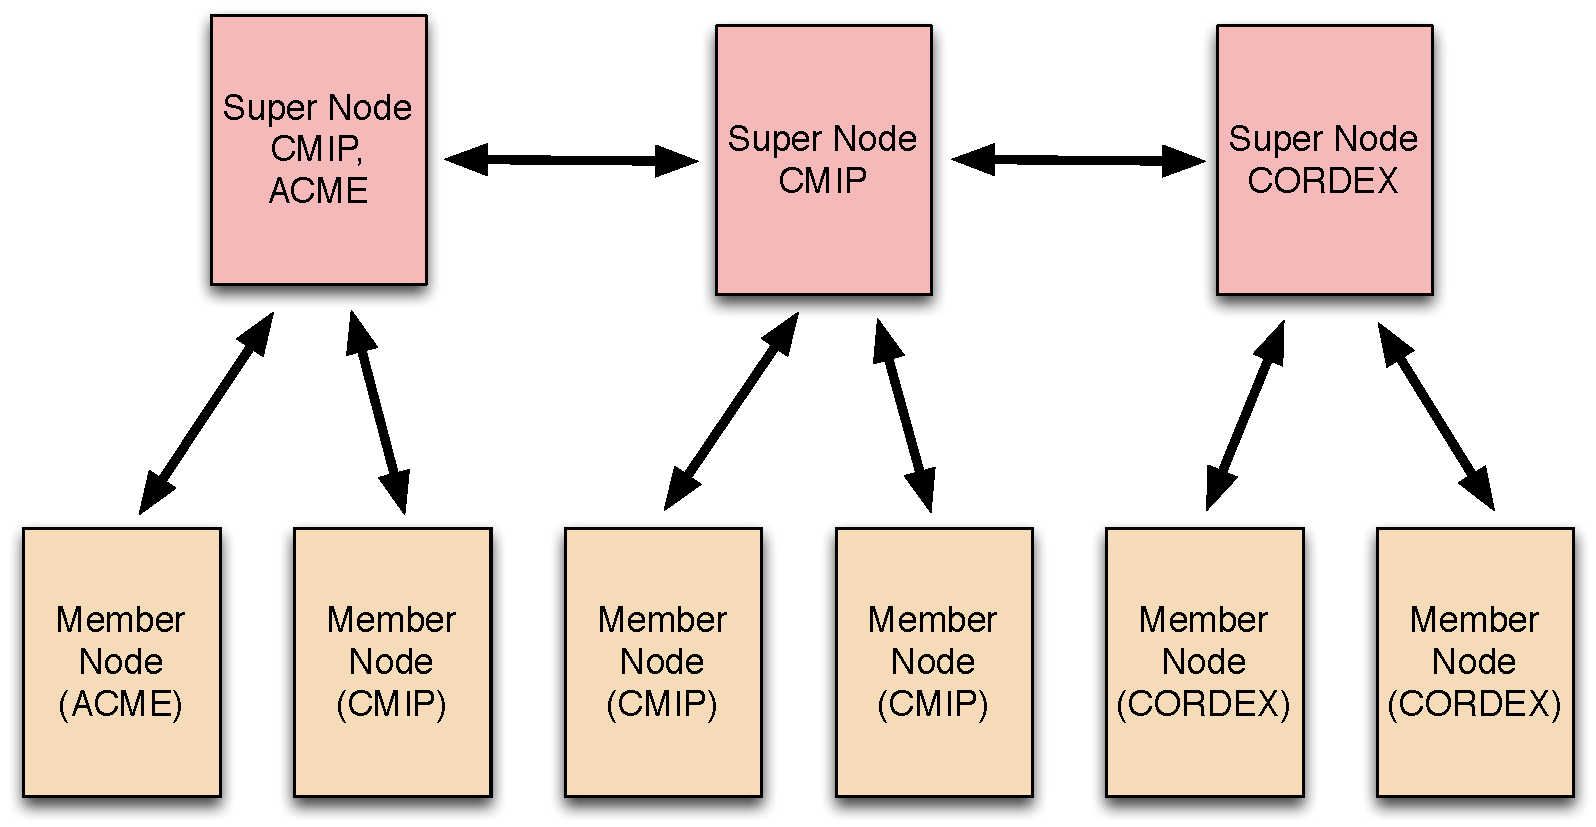
\includegraphics[width=\textwidth]{presentation/ESG-node-org.pdf}
Figure 3: SuperNodes and member nodes belong to project organizations and share project-specific information.   Multiple SuperNodes that coordinate service configuration specific to a project will share information among each other, but not with a SuperNode for a different project.  Example of such configurations include project specific settings for publication and access control.
\end{center}

\section{System Design}
\label{sysd}

"Minimum Spanning Tree"-based node communication among SuperNodes for content consistency updates.  Communication among peers is deterministic based on a node assigned number (taken from the master list of SuperNodes).     Standby nodes are assigned potential slots in the event they become activated so each know who the peers will be.  Standby nodes function as member nodes, so these nodes have been assigned a SuperNode and that SuperNode is independent of where the standby nodes will reside in the tree overlay network structure for SuperNode communication.  Member nodes are shown attached to nodes \# 3 and 4 in this example (Figure 4).  However all SuperNodes are expected to have some assigned member nodes, but not essential.  SuperNodes can still function in a relay role without any member nodes and may be needed to take on member nodes as soon as another fails or imbalance occurs. 

\begin{enumerate}
\item The comprehensive list of SuperNodes is manually updated in the controlling git repository, which also contains global configuration parameters for SuperNodes; ex: maximum number of membernodes that can be serviced by SuperNode etc
\item When a new node is brought up, it fetches the list of SuperNodes and starts communicating with each of them, in sequence, till it contacts a SuperNode that admits the member node. When a new node contacts a SuperNode for membership, these are the possible results:
\begin{enumerate}
\item \textbf{No response}: if SuperNode is down or unreachable.
\item \textbf{Deny}: if the contacted node is no longer operating as a SuperNode or if the SuperNode is already fully subscribed.
\item \textbf{Accept}: if the SuperNode agrees to serve it.  This is a slightly "delayed" response as the SuperNode must check with others in event of a reassignment lock. 
\item \textbf{Delayed Accept}:  There is a reassignment in progress, and the node should wait a short while before contact this or other SuperNodes. 
\end{enumerate}
%\item SuperNodes establish project group ZK-node directory instances.  Each project includes the min and max thresholds for SuperNode count.  The threshold may increase if a larger number of project nodes join a group.  We expect that these settings will initially be controlled by a SuperNode administrator, but could be automated.


%\item Super and Member nodes establish ephemeral nodes for project group membership.  Based on the property of ephemeral nodes, an instance will not persist if a creator Member Node becomes unavailable.  The ephemeral node instance contains the high-level characteristics for the node, such as the node types running (data, index, idp, compute),  maybe user, data set counts, other projects hosted.  
%\item Standby nodes set their status in a subdirectory for the project group

%\item the first standby node will assume SuperNode responsibility if the project SN count threshold dips below the minimum allowed.  A thread in the node manager service may poll the ZK ephemeral nodes to see if the change over is required, then can invoke the SN role library functions.


\item SuperNode legacy service for registration.xml pulls node "alive" information to feed to the Dashboard.  

\end{enumerate}
\begin{center}
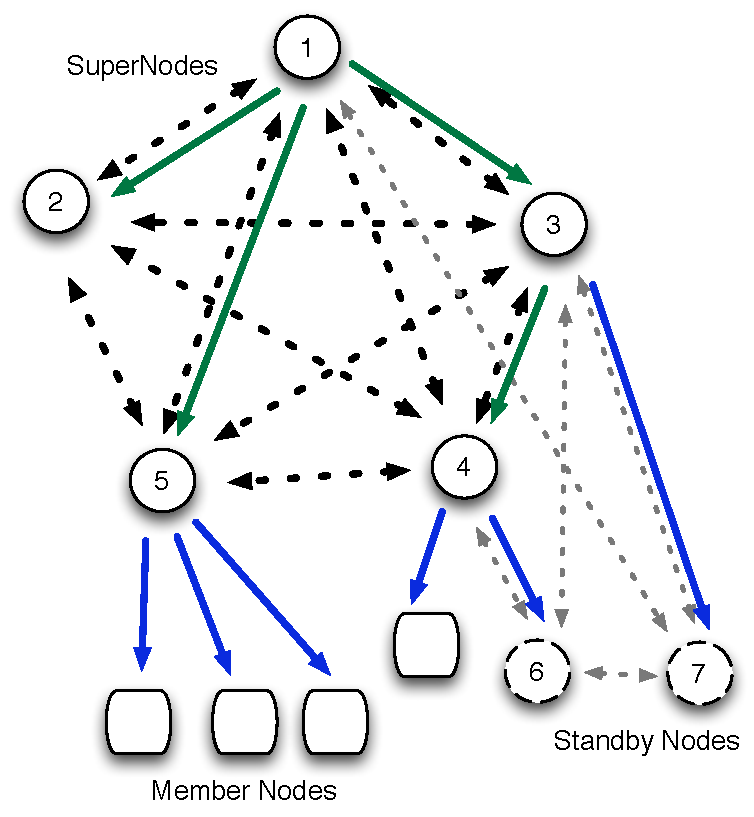
\includegraphics[width=5in]{presentation/Node-comm-v3.pdf}\\
Figure 4: node manager communication.  Black dashed arrows show health check $(n^2)$.  Gray dash represent addition of standby nodes (which under normal circumstances are member nodes).  Dark blue arrows show SuperNode to member node queries.  Dark green shows minimum spanning tree overlay for update propagation.
\end{center}

%\subsection{Member Node reassignment}
\section{Communication Design}
\input{commdesign}
\subsection{Member Node reassignment}

In the event that a SuperNode becomes unavailable, the managed member nodes must be assigned to other SuperNodes temporarily.  The strategy to complete this is a greedy algorithm based on the number of nodes to be assigned, and the ranking of SuperNodes from lowest to greatest available load.  The load information is agreed upon by the tree-based communication prior to assignment.  Disagreements must be resolved.  Additional nodes wait to join the federation until the reassignment is complete. 

Strategy 2:  greedy algorithm based on latencies.  Member nodes are assigned to SuperNodes using lowest latency in a similar greedy algorithm.  The measuring of latencies is performed as an infrequent periodic check based on the current node map (daily/weekly?)




\section{Authentication mechanisms}
Distinction to be made between user authentication and system authentication, as certain privileged operations may need to be executed without human intervention. This would need a system or process to be authorized to perform the operation. 




\section{API Specification}

There are two APIs provided by the node manager.  First is the node-to-node client/server API.  Second is the node manager service API used on the node.  Requests that involve forwarding are held in queues, so they can wait until a communication problem is resolved. 

\subsection{Node-to-Node API}

The API is available as URLs (over apache). The node manager uses the built-in python http client to connect to a remote server

\begin{enumerate}
\item
SuperNode Health check request.  Parameter(s): list of edges.  Responds with ack for self.  SuperNode "bootstrap" to initiate a federation uses this method as well, but the message content varies to reflect the distinction. 

\item
Health check delegation response.  Contains the point to point connections that have been validated, and/or health of reachable nodes.

\item
Member node Health check:  Response: Healthy, Unhealthy with failed services
\item
member node metric query.
\item
Status push to member node.
\item
Component metadata/configuration push.  Uses the established communication map.  If a (SuperNode) is unreachable, the request stays in a queue until the node is detected as reachable.  Member nodes will receive delayed updates from new SuperNode
\item
Communication map push.  Originates on temporary leader node.  Recipient branch nodes forward to their neighbors as designated.
\item
Standby node to SuperNode delegation.  Response: acknowledgement or in immediate unhealthy state.
\item
Member node reassignment request.  Performed by the SuperNode (standby) taking over member nodes whose normally designated SuperNode is unreachable.   Similar message used when the old SuperNode resumes its duties.
\item
Member node reassignment acknowledgement.  This is sent to the new SuperNode.
\item
Data versioning consistency checks.  SuperNode to SuperNode checks use the MST; SuperNodes check against their member nodes. Outdated versions are corrected by a point-to-point update.  If a versioning conflict arises, nodes roll back to the previous consistent version until the conflict can be resolved by administrators.
\item
Member node admission request (see \ref{sysd}).   
\item
Member Node decommission. 
\item 
Temporary SuperNode removal for maintenance.  (Note that SuperNode decommission, a more permanent action, takes place via [1] removal from the list [2] reinitialization of SuperNodes via bootstrap protocol.

\end{enumerate}

\subsection{Service API (within a single Node)}

The Service API is the API that other software modules running on ESGF nodes may use to access federated information managed by the Node Manager.  An example is the publisher can use the API to put configuration metadata into the federation to be shared among other member nodes.  We present Several alternatives for this API: first, what sort of interface is available (methods); second how (what means) of connection would modules have to access the API.\\
\\
 The simplest API would allow each component to read and write an ASCII blob; thus completely unstructured data from the perspective of the Node Manager.  The node manager would keep such a config for each component for each project that the node participates.   Any structure would be the responsibility of the client to serialize, e.g. json objects.  \\
 \\
 This information is collected and disseminated on a \emph{per project} basis.  Nodes that serve as SuperNodes for particular projects are the sources for shared configuration information, while member nodes that subscribe to particular projects are the recipients of specifically those projects info (multiple are permitted).
 
 We envision the following methods to this API:
 
 \begin{itemize}
\item
\textbf{Register:}  run as a ``bootstrap'' to set up a new client (ESGF component) / project entry.
Registration has two phases:  \begin{enumerate}
\item
Component registration:  invoked as part of the ESGF / component installation once components are upgraded to integrate with the Node Manager for the purpose of federated configuration management.  
\item
Project registration: can also occur during installation.  If a node joins an additional project after installation, an administrator tool e.g. "esg-node" can update the node manager to add the project.
\end{enumerate}
 \item
 \textbf{Put:} For a particular new client (ESGF component) / project entry, add/update a ``blob'' of data
\item

\textbf{Get:}  Retrieve the blob.
\item
\textbf{Delete}  Removes the blob (Need a use case for this)
   
   \end{itemize}
   
    JSON objects can be build using python dictionary and list constructs, and so are straightforward to encode and store in the node manager serving as repository for the data blobs under the API.   Services configured at the project level are done normally via a SuperNode admin and propagated to other SuperNodes and the member nodes.  A more in-depth alternative would be to allow for key-values to exist within the API.  Thus, the node manager could serialize a dictionary for each.\\
\\
The stored items are versioned.  Versioned items should be consistent.  Periodic checks are performed.  We anticipate with proper access control, prescribed workflow for changes, and sound project governance, conflicts due to simultaneous update will be kept to a minimum.  An option would be for the repository to be updated via \emph{git} to handle conflict resolution rather than maintained via node manager based updates (see Conflict Resolution).
When using git, the SuperNodes would send messages to others informing of a change, but not the specific contents of that change.  The recipient nodes would pull the change from the git repo.  
\\
\\

\subsubsection{API Interface Style}

There are several alternatives for means of connection with the API:

\begin{itemize}
\item \textbf{Python API for direct access to files:}  While we expect that most applications will not make frequent changes in the case of configuration, this mode of access is not desirable.  Nonetheless, its feasible for a component to import the internal api, or directly modify the underlying store.  There could be on-node and off node synchronization issues.  On node if the node manager in-memory copy becomes out of sync if another process makes a modification.  
\item Write to task queue. This option would not have the synchronization issues, as the node manager would make the updates.  The calling application must be configured with the settings for the task queue, which is most likely ok, but somewhat less abstract
\item Task queue wrapper library.  The library has the task queue settings.  This is similar to what is done within the node manager internal for Django url listeners.
\item ``localhost'' http connections.  Use urls for the node manager.  This makes the API similar to the node-to-node API.   Localhosts need to know how to construct the urls, attach data. (The current prototype uses GET).  A drawback is a potential security hole that external nodes can access as well as local connections. 
\item Wrapper library around urls.  Abstracts away the url syntax and http connection semantics.  We may be able to add some security, e.g. shared secret on localhost that external nodes would not have.

\end{itemize}

\subsubsection{URL security solutions}

Several alternatives:

\begin{description}

\item[Shared Secret] The secret can be generated on the node during install, perhaps a hash derived node name, local time, phrase input, etc.  The client would need to present the secret to the API, which upon validation would process  requests, otherwise reject them.  This would allow an administrator access to the secret for troubleshooting using an external client.
\item[Alternative Port]  Run on a port inaccessible off node, ie. removed via iptables and/or blocked via firewall.  localhost:port connections would still be valid.  
\item[Incoming IP filtering]  Establish the django listener to only accept local connections.  Testing is possible with browser running on localhost.

\end{description}

We can a use a combination of these.

\section{Conflict Resolution}

Conflicts may arise due to some race conditions.  The most likely scenario is that a SuperNode is added around the same time that another one goes down (temporarily).    This problem can be problematic if the messages regarding these events arrive out of order.  A symptom is that member nodes are getting mixed messages or multiple SuperNode reassignments.  
  The task manager on each SuperNode keeps a record of the timestamp of the latest task.  If a task arrives that is stamped earlier than the latest (or in unlikely event of a tie, has a greater id stamp; the smaller node id that generated the message breaks unlikely ties), then the node needs to replay the log. 
  The SuperNode will store the file followed by $N$ histories in a "journal" back a period of $T$.  
    The node needs to check for duplicated messages over this period.  Moreover, all messages should be assumed that duplication is possible.  Thus, either implement checks in a history, or check if the message would become meaningless based on the state.  Eg, member nodes already have valid assignments.   The hope is that these conflicts work themselves out after minutes, so patience is required on the user's part. \\
    \\
   For instance, in terms of how this may become an issue in practice, consider a SuperNode forwarding an update message creates a separate thread to communicate with others regarding a change.  Because the change occurred in time on the original server, it has been assigned a timestamp.  Due to load on the server, that thread does not get to run for seconds and when it is finally set to run, the timestamp is earlier than another event.  So when the communication occurs, the event is written after an event with a later timestamp.  The recipient node catches this and then replays the log.   \\
 
    
\begin{center}
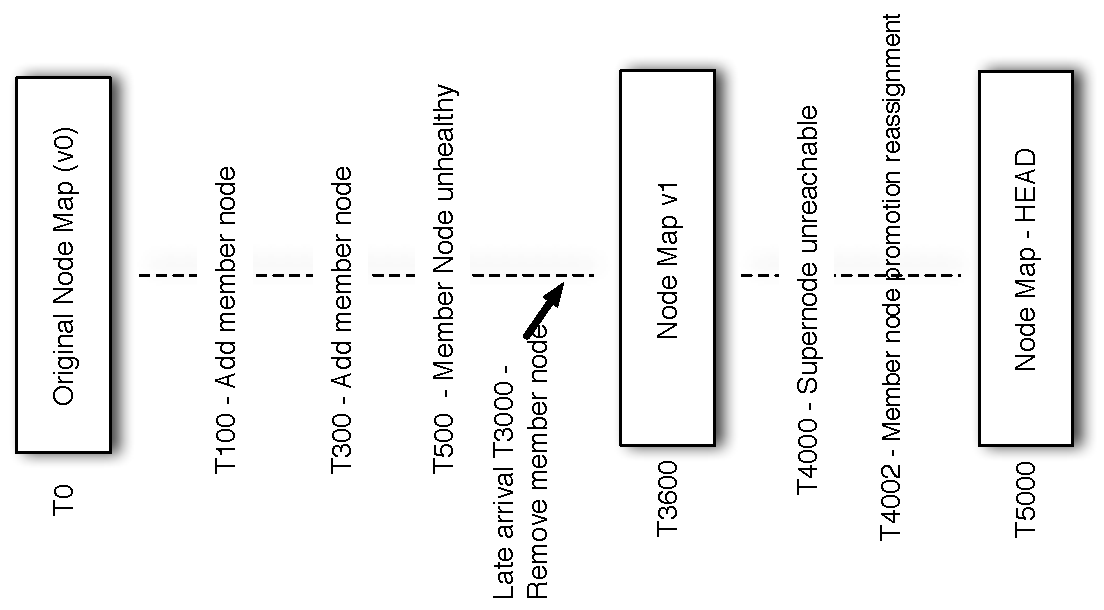
\includegraphics[width=\textwidth]{presentation/timeline.pdf}
Figure 5: Events timeline for node map with versions.  Inserting a late event forces a replay of the timeline from the previous version of the event.  V1 will become invalidated in this example. 
\end{center}

\section{Breakup of tasks}

\subsection{Communication}

\begin{enumerate}
\item
Review AVL tree reorganization
\item
Model deterministic communication
\item
Measurement of node to node latency.  This is needed for all member nodes to all SuperNode.  TBD  needed for member node - member node, SuperNode 
\item
Use django test web server as a prototype for setting up a test api for health check and other component services.
\item
Investigate task management, worker queue, etc.  frameworks.  For prototyping we can implement python threads with polling/locks on shared objects.  The health check initiator can run as its own process.  Threads needed to manage incoming requests and assemble a node map.  Celery is a well-know queue API, but bases on RabbitMQ.  There are other alternatives implemented but no standard.
\item
Integrate with Apache using proxy setup.  Run on some port in a python virtualenv.


\end{enumerate}


%\subsection{zookeeper evaluation}
%\begin{enumerate}
%\item
%Performance evaluation
%\item
%Evaluate functionality
%\item
%Assess  API
%\end{enumerate}

\subsection{Metrics gathering}
\begin{enumerate}
\item Investigate logger issue
\item Decouple logger from Node Manager
\item Ensure generation of registration.xml
\end{enumerate}

\subsection{Administrator Console/Interface}
\begin{itemize}
\item
Currently handled by esg-node
\item
What items for SuperNode?
\item
What for member nodes?
\item
Shared items, e.g. project membership
\end{itemize}



\section{Issues and questions}
This is to be a place to list out problems that need to be handled.
\begin{enumerate}

\item
Need to determine in which circumstances using \emph{git} as a "Super Repository"  for config data for purposes of reliability and consistency is appropriate.
\item
Settle on the particular interface style for the API.  We are leaning toward local http connection, but need to decide on a technique for securing the API to local connections.

\item
Deal with "spoofed" node; ensure relayed information is legitimate. 
\item
%Need to choose centralized query service database system.  Use Hadoop, spark, Hive, Cassandra, or some RDBMS?
Need the SuperNode to query nodes for metrics and perform aggregation where necessary.
\item
Should all SuperNodes in ESGF participate in $n^2$ health check scheme regardless of project? Given that we expect the data centers to service multiple projects and likely contain several SuperNodes, we favor this approach rather than have each have the burden of a per-project health check for some SuperNodes.
\item  Use of Django/Work queue framework.  Django handles incoming connections over http.  However, associated tasks happen in the background.  They need to be pushed off to separate threads if in same process space.  If separate node manager process, need a IPC mechanism.  Easy IPC can happen through a shared directory where files represent tasks and are produced/consumed.  The django "listeners" become the task producers and a single python process is the consumer.   Python can fork threads for tasks that should occur asynchronously, but update to state must be synchronous as some of the scenarios involve merging updates from multiple nodes.
\item
For what specific information should the Node Manager rely on the PostgreSQL database for storage?


\end{enumerate}

\section{To revisit}
\begin{enumerate}
\item Support for automated replication of datasets
\item Support for an update manager service (to supplant present esgf-installer)
\item Metrics collection: what needs to be done for aggregation? Does it clash with what Sandro intends to do?
\end{enumerate}
%\nocite{KandR


%\appendix
\begin{appendices}


\chapter{Feedback and questions from the F2F 2014}
\begin{enumerate}
\item Can ZooKeeper be proxied on http/https, to avoid having to open up further ports.
\item Can the \nm implement federated attribute service?
\item Luca's virtual organization management vs project level management by \nm How do they fit in ?
\end{enumerate}



\chapter{ZooKeeper Questions}
Kept for posterity, as our evaluation of ZooKeeper showed that it had the desired functionality for many of the consistency needs.  In event we decide to revisit, we have a point of reference. 
\begin{enumerate}

\item
Do we use zookeeper?
\begin{enumerate}
\item \redline{Implementing dynamic changes by adding or removing ZKs might be problematic.}
\item \redline{ZK seems to be designed to operate behind a firewall, preferably with all hosts on the same subnet.}
\item \redline{ZK not designed with focus on security, as common implementations are cluster management etc, all behind firewall}
\item \redline{Getting hosts to open up additional ports is cumbersome and a backward step} 
\end{enumerate}
\item
To what extent can we rely if we do,  what do we need to implement for the \nm?

Is zookeeper a fit for management?
\item
Can zookeeper manage group-level access control?  We think it can.  Need to evaluate.
\item
Is zookeeper python API adequate?
\end{enumerate}
\end{appendices}
\printbibliography
\hypertarget{mymarker}{}
\printindex
\end{document}
